\chapter{LaTeX Docker \\
\small{\textit{-- Ivan Farfan, Johan Jaramillo, Ryan Davis}}}
\index{latexdocker} 
\index{Chapter!LaTeXDocker}
\label{Chapter::LaTeXDocker}

\section{Project Layout}
Create a folder with these files:
\begin{minted}[fontsize=\small,breaklines]{text}
.
├── Dockerfile
└── main.tex
\end{minted}

\section{Dockerfile}
This Dockerfile installs TeX Live and sets up a container to compile LaTeX.

\begin{minted}[fontsize=\small,breaklines]{docker}
FROM debian:bookworm-slim
RUN apt-get update && apt-get install -y \
    texlive-latex-base \
    texlive-latex-recommended \
    texlive-latex-extra \
    texlive-fonts-recommended \
    latexmk \
    python3-pygments \
 && apt-get clean && rm -rf /var/lib/apt/lists/*
WORKDIR /data
CMD ["latexmk", "-pdf", "-shell-escape", "main.tex"]
\end{minted}

\section{Build and Run}
\begin{minted}[fontsize=\small,breaklines]{bash}
# Build the Docker image
docker build -t latex-docker .

# Run the container (Linux/macOS)
docker run --rm -v $(pwd):/data latex-docker

# Run the container (Windows PowerShell)
docker run --rm -v ${PWD}:/data latex-docker

# Run the container (Windows CMD)
docker run --rm -v %cd%:/data latex-docker
\end{minted}
\section{Screenshot}
The following screenshot shows the result of compiling our LaTeX document inside
the Docker container.

\begin{center}
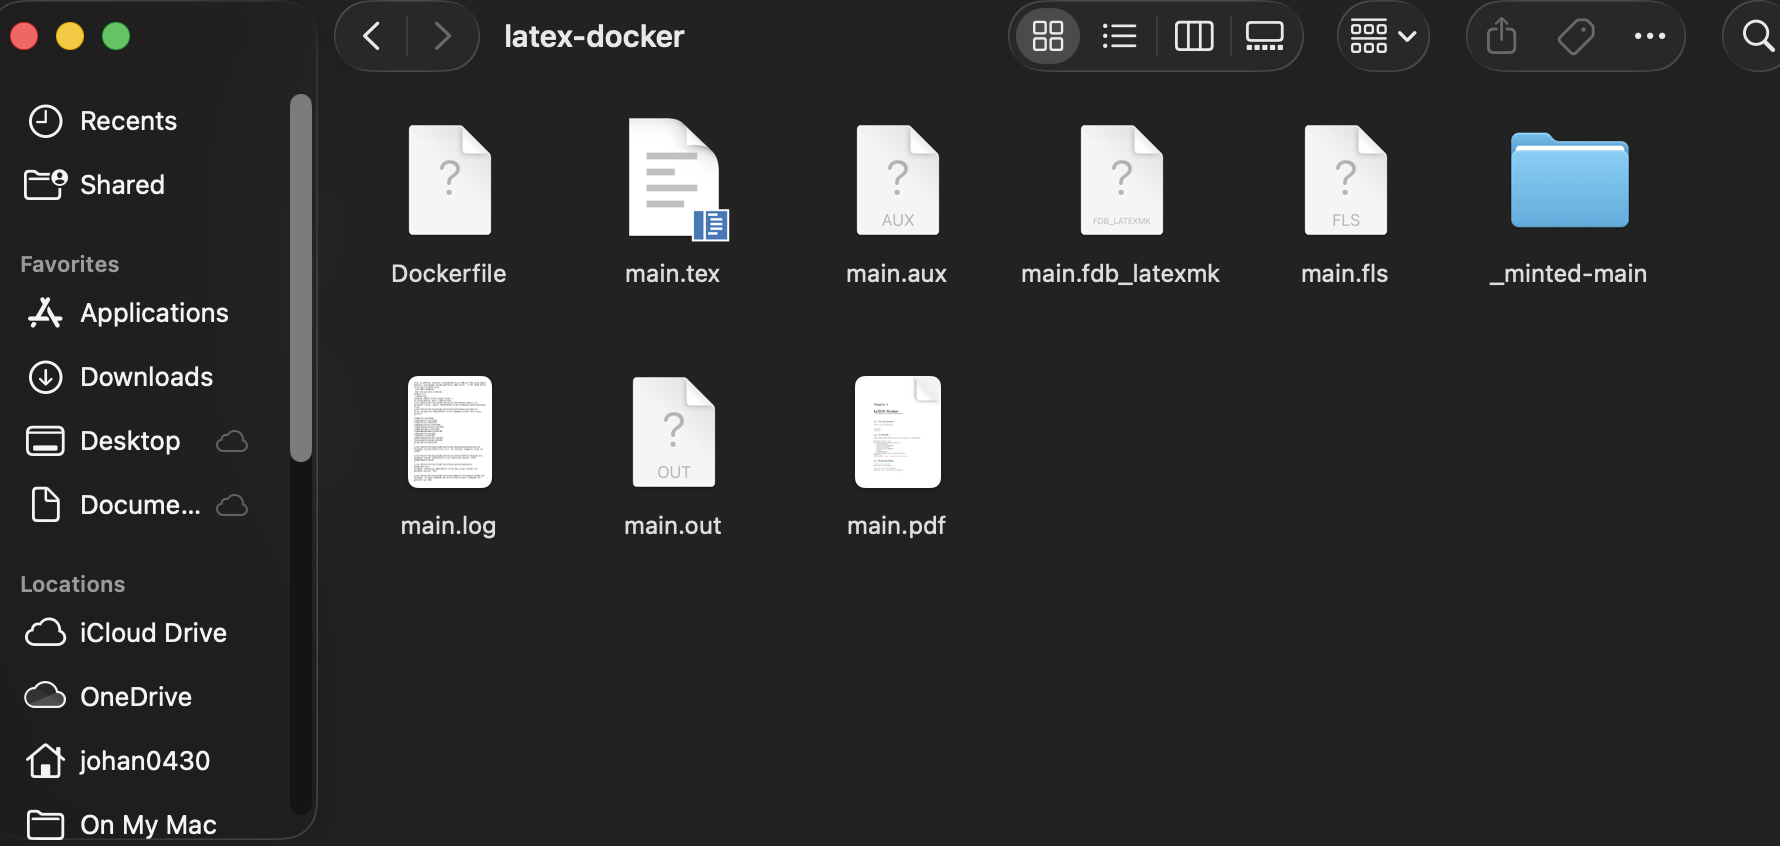
\includegraphics[width=0.9\textwidth]{png/latexdocker.png}
\end{center}


\section{Conclusion}
In this chapter we showed how to use Docker to build a container that can
compile LaTeX documents with TeX Live. The steps included writing a Dockerfile,
setting up the folder structure, and running basic commands to build and run the
container. This setup is similar to how Overleaf works behind the scenes. Even
though our example was simple, it demonstrates how Docker can make LaTeX
compilation consistent and portable across different systems.